%=====================================================
%====== If you are new to LaTeX, this website ========
%======     will be your new best friend:     ========
%======   http://en.wikibooks.org/wiki/LaTeX  ========
%======   Template created by Jonathan Blair  ========
%=====================================================



%=====================================================
%============ Controls ===============================
%=====================================================

%\documentclass[12pt,letterpaper,onecolumn]{article}
\documentclass[11pt,letterpaper,onecolumn]{article}
%\documentclass[10pt,letterpaper,onecolumn]{article}  % not recommended
%\documentclass[12pt,letterpaper,twocolumn]{article}
%\documentclass[11pt,letterpaper,twocolumn]{article}
%\documentclass[10pt,letterpaper,twocolumn]{article}


\usepackage{amsmath}
\usepackage{graphicx}
\usepackage{url}
\usepackage{textgreek}
\usepackage{float}
%\graphicspath{{path-to-folder-containing-necessary-graphics}{other folder as necessary}}


%=====================================================
%============ \begin{document} =======================
%=====================================================

\begin{document}

%=====================================================
%============ Title ==================================
%=====================================================

\title{\bf Behavior of the Shockley Equation at Various Temperatures}
%\title{\Large\bf Larger, Bolded Title}

%=====================================================
%============ Author =================================
%=====================================================
\author{
 Jairo Portillo \\*
  \\*
 PHY 353L Modern Laboratory \\*
 Department of Physics \\*
 The University of Texas at Austin \\*
 Austin, TX 78712, USA
}
\date{September 28, 2015}

%\address{The University of Texas, Austin, Texas, 78712}

\maketitle

%=====================================================
%============ Abstract ===============================
%=====================================================

\begin{abstract}
A silicon diode was exposed to various temperature conditions in order to observe
the relation of current ad a function of voltage. We compared our observations to
the Shockley Equation on order to confirm the behavior of the diode. Our
observations experienced an exponential curve and confirm the behavior expected of
a semiconductor predicted by the Shockley Equation.
%$I = I_S (e^\frac{qV_D}{nkT}-1)$$ 

\end{abstract}

%=====================================================
%============ Body of the article ==========================
%=====================================================

%=====================================================
%============ Section ==================================
%=====================================================

\section{Introduction}

\subsection{Physics Motivation}

Intrinsic Semiconductors are crystal lattice structures that have a small energy gap between the valence band and the second highest band compared to that of an insulator. A p-n junction semiconductor uses two opposite doped semiconductor regions forming a diode. The n-type (negative) semiconductor is doped with atoms that have one more outer electron than the intrinsic semiconductor, while p-type (positive) are doped with atoms that have one less electron. The difference in charge allows the electrons and holes to diffuse. The diffusion of electrons leaves exposed charges that are immobilized in the lattice. This causes an electric field that forms a depletion region, which is absent of free electrons, in between the p-type and n-type.~\cite{Hons,Roh,Bart} 

In this case the diode was in a steady state, that is a constant voltage is being applied over the diode and under forward and reverse bias. Forward bias occurs when the positive terminal is connected to the p-type and the negative terminal is connected to the n-type. This reduces the electric field and allows carriers to flow and can be described by the Maxwell-Boltzmann distribution. Reverse bias occurs when the negative terminal is connected to the p-type and the positive terminal is connected to the n-type and restricts the flow of carriers but allows diffusion. The sum of the currents of the forward bias and reverse bias gives us the Shockley equation.~\cite{Roh}

Diodes, specifically p-n junctions, are important to modern electronics. The Shockley equation, which describes the behavior of diode, was developed by William Shockley, a founder of modern transistors. A component in nearly all electronic especially computers.

\subsection{Theoretical background}

The Shockley Equation that models the total current of a diode

{\Large$$I = I_0(e^\frac{qV}{nkT}-1){\normalsize,}$$}

where I is the net current flow, $\mathrm{I_0}$ is the saturation current, q is the absolute value of the electron charge, V is the voltage across the diode, n is the ideal factor and is between 1 and 2 but will be assumed to be 2 in this experiment, k is Boltzmann's constant, and T is temperature.

The saturation current is a representation of the recombination in the diode and is also influenced by temperature.  This recombination is occurs with the movement of electron and holes. As seen by Rolhf, the saturation current is dependent of the sum of the current of electron from the n-region to p-region and current of holes moving from the p-region to n-region. The variations of temperature influence the impurity atoms that give the junctions their charge. The colder the diode, the more likely electrons will bind to the impurity atom. The hotter the diode, the less likely electrons will bind to the impurity atom. The vibrations of the impurity atom are what prevent the electron from binding.~\cite{Hons,Roh,Shock}  

\subsection{Our approach}

In order to observe the properties of the p-n junction, we simply had to apply a voltage across the diode and measure the current. Other properties could also be observed by altering the temperature of the diode. One method this can be done as noted by Mesissinos and Napolitano is to attach a diode to a copper plate with conductive epoxy and attach a resistor on the other side to use as a heat source with a thermocouple to record temperature. With this method.~\cite{EMP}

We set up a similar circuit as to that referenced by Mesissinos and Napolitano but in order to vary temperature, we used heat shrink to protect the diode from various elements. The diode was tested at room temperature (296.8 $\pm$ 1.4K) , in steaming water (367.7 $\pm$ 4.2K), and liquid nitrogen (70.1 $\pm$ 7.1K).

%=====================================================
%============ Section ==================================
%=====================================================

\section{Experimental setup}

\subsection{Apparatus}

The picture of the setup in Mesissinos and Napolitano was very ambiguous, so we had to design our own circuit. At first we had the voltmeter in series with the diode and the Keithley picoAmmeter in parallel with the voltmeter and diode. It came to out attention that the resistance in the voltmeter was drastically altering our current measurements as compared to it not being in the circuit. We then placed the ammeter in series with the diode and the voltmeter in parallel as seen in Figure~\ref{fig:cir}.This gave us reliable results as we did not have to account for the resistance of the voltmeter. We varied the temperature by exposing the shrink wrapped diode to steaming water and liquid nitrogen in appropriate containers. 


%=====================================================
%============ Importing pictures  ==========================
%=====================================================

% !! To be imported, all graphics must be converted !!
% !!    to encapsulated postscript (.eps format)    !!
% !!  The GNU Image Manipulation Program (GIMP) is  !!
% !!          capable of this conversion.           !!

\begin{figure}[H]
  %
  % placement specifier = { h,t,b,p,!,H }
  % see the following url for placement specifier definitions:
  % http://en.wikibooks.org/wiki/LaTeX/Floats,_Figures_and_Captions
  %
 \begin{center}
 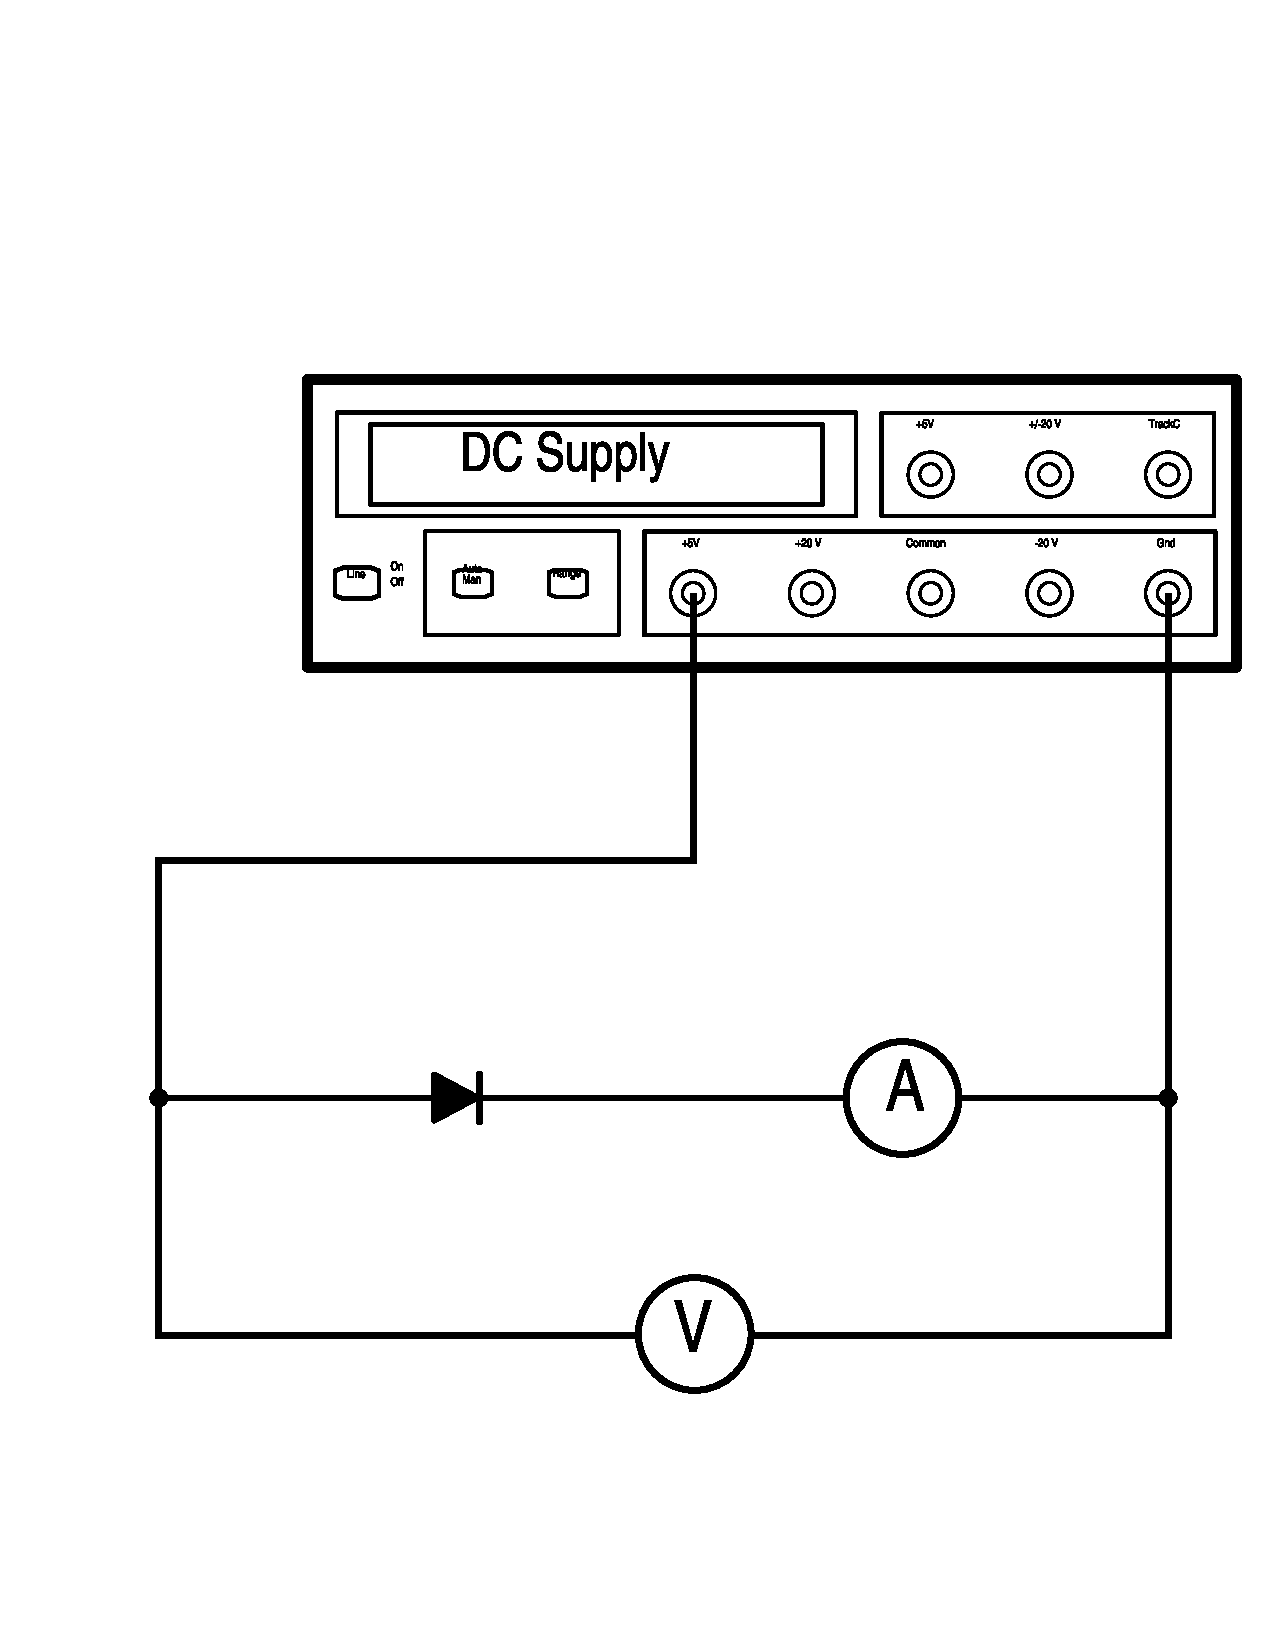
\includegraphics[scale=.25]{Circuit.pdf}
  %
  %               [llx,lly][urx,ury]{ filename.eps }
  %
  % Note: llx = lower left x coordinate
  %       lly = lower left y coordinate
  %       urx = upper right x coordinate
  %       ury = upper right y coordinate
  %
  %       If [ llx,lly ] is omitted, [0,0] is assumed.
  %       Be sure to include units.
  %
 \caption{ Our parallel circuit design.\label{fig:cir} }
 % See http://en.wikibooks.org/wiki/LaTeX/Labels_and_Cross-referencing
 %  for information on labels.
 \end{center}
\end{figure}



\subsection{Data Collection}
\begin{figure}[H]
  %
  % placement specifier = { h,t,b,p,!,H }
  % see the following url for placement specifier definitions:
  % http://en.wikibooks.org/wiki/LaTeX/Floats,_Figures_and_Captions
  %
 \begin{center}
 \includegraphics*[scale = .9]{TempComp.pdf}
  %
  %               [llx,lly][urx,ury]{ filename.eps }
  %
  % Note: llx = lower left x coordinate
  %       lly = lower left y coordinate
  %       urx = upper right x coordinate
  %       ury = upper right y coordinate
  %
  %       If [ llx,lly ] is omitted, [0,0] is assumed.
  %       Be sure to include units.
  %
 \caption{ This a plot of all three temperatures with current as a function of voltage. The diode demonstrates behavior predicted by the Shockley equation.~\label{fig:all3} }
 % See http://en.wikibooks.org/wiki/LaTeX/Labels_and_Cross-referencing
 %  for information on labels.
 \end{center}
\end{figure}

The voltmeter was used to determine the applied voltage and was measured at a consistent interval. Since the hot plate used to heat the water did not have a digital reader thermometer was used to determine the temperature. This took some time as we had to adjust the hot plate until the thermometer had a fairly stable reading. A Keithley picoAmmeter was used as the current reading ranged from milliampere to nanoampere. In order to obatain the best data, the average function was used on the ammeter which averages a number of previous measurements that one sets in order to relay a more stable measurement. For room temperature and the steaming water, we averaged 20 readings for each voltage and for liquid nitrogen we averaged 50. 50 reading were used for liquid nitrogen as it had the largest and most unstable measurements, this was an attempt to maintain a small error. In order to measure the saturation current, we simply reversed the leads in order to place in diode into reverse bias. 



%=====================================================
%============ Section ==================================
%=====================================================

\section{Data Analysis and Results}

\subsection{Data Processing and Hypothesis Testing}
\begin{figure}[H]
\centering
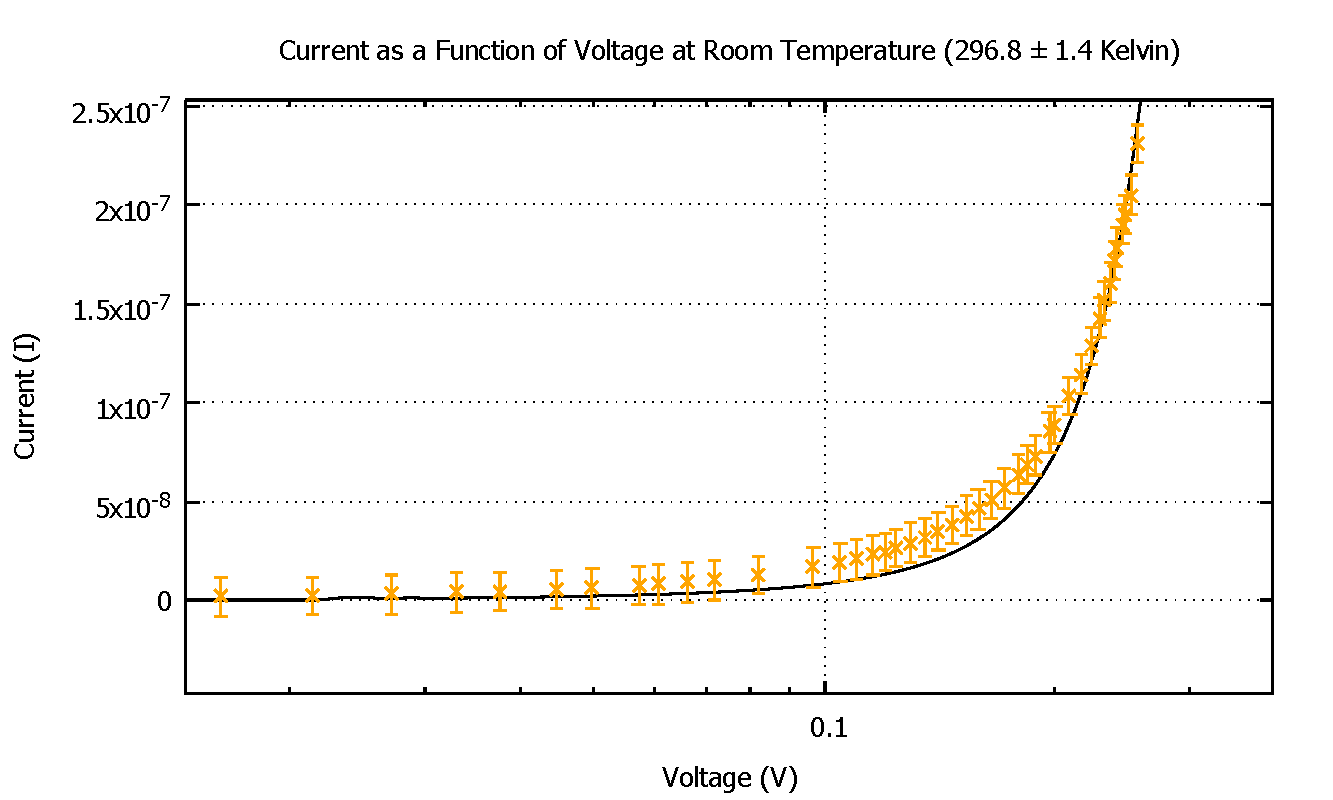
\includegraphics[scale =.5]{RoomTemp1.pdf}
\caption{The Room Temperature plot of current as a function of voltage with its fit curve and error bars.\label{fig:rmtmp}}

\end{figure}
\begin{figure}[H]
\centering
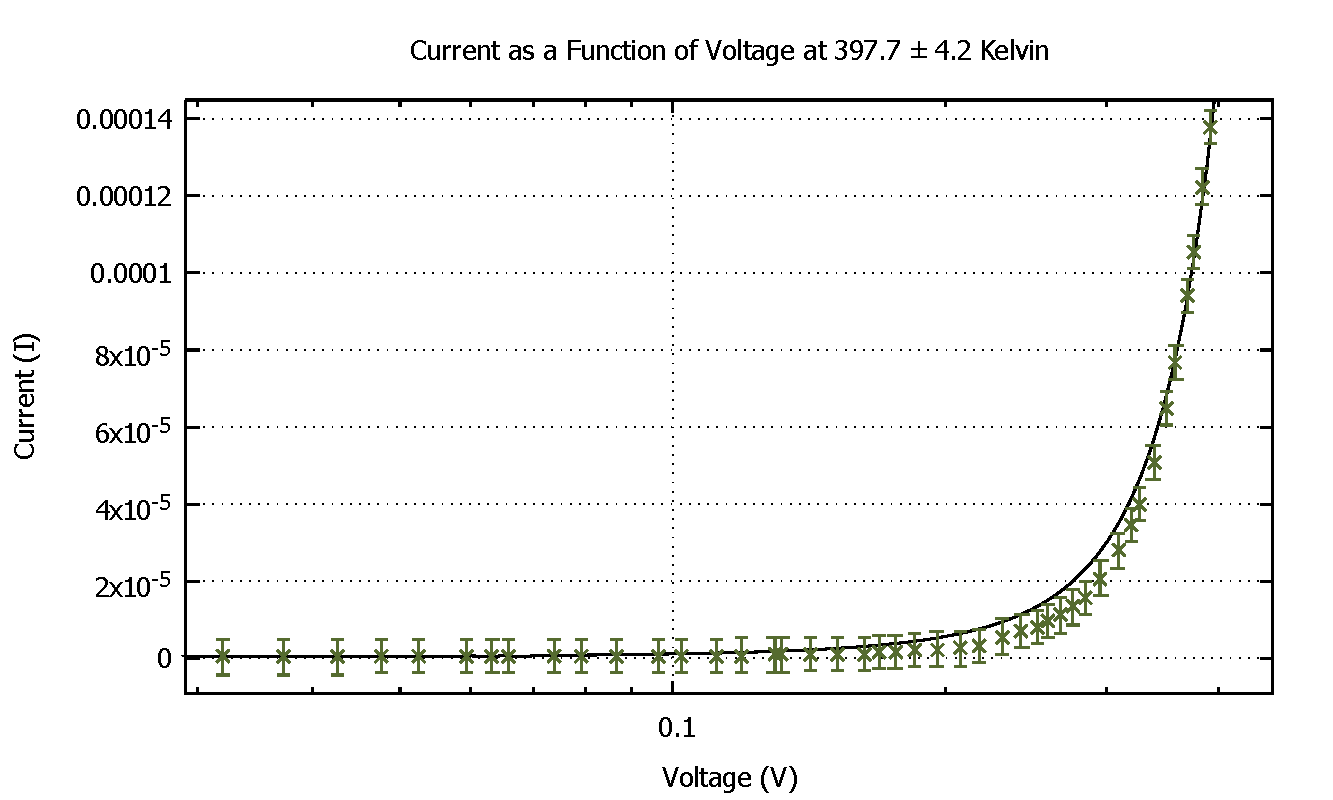
\includegraphics[scale =.5]{HotTemp1.pdf}
\caption{The Steaming Water Temperature plot of current as a function of voltage with its fit curve and error bars.\label{fig:htmp}}

\end{figure}

For all three temperatures, a fit to the Shockley equation was done in the same form as above and only allowing the saturation current to change in the fit. Limiting the fit to one parameter did not seem ideal until after it was done except for the liquid nitrogen plot.

In order to find a good fit, we used the average of the currents in reverse bias. For room temperature, the initial guess for the saturation current was 3.635nA  $\pm$.717$\mu$A with room temperature current with an error of $\pm$9.789nA. The fit gave us a saturation current of  $\text{V}_\text{T}^{-1}$. As seen in Figure~\ref{fig:rmtmp}, the data falls right along the fit curve. For the 367.7K, the average saturation current was 22.09pA $\pm$.764 $\mu$A. The fit for the 367.7K gave .2025$\mu$A $\pm$.216pA. Figure~\ref{fig:htmp} shows a similar pattern as the room temperature plot. The plots also exhibit the shift due to the temperature fluctuation as seen in Figure~\ref{fig:all3}. 

The liquid nitrogen plot was unable to have a valid fit depending solely on the saturation current. The exponent in the Shockley equation would explode reaching values in the teraAmps within our voltage range. It was found that $\frac{q}{kT}= \text{V}_\text{T}^{-1}$, which is simply the inverse thermal voltage, can not be $10\%$ to $20\%$ off from 39$\text{V}^{-1}$ or the fit will fail as stated by William Shockley. The $\text{V}_\text{T}^{-1}$ for liquid nitrogen was 165.5 $\pm$ 12.3$\text{V}^{-1}$ which is about 300$\%$ off.~\cite{Shock} 

A major source of error was the fluctuations in the measurements from the ammeter. Though using the average function did help clear some noise, it made the data collecting process that much longer and tedious as there were still fluctuations. Another error and likely contributed to the fluctuations was the diode was connected into the circuit with multiple wire segments rather that one long wire for each side. This may have has poor contact thus affecting the current flow. This was noted as when pressure was placed on the contacts, the current measurement would rise. However through out the experiment no pressure was added to the leads which leads us to assume our data is consistent. A final source of error one, that was not noted during the experiment, was the time it took for the diode to achieve thermal equilibrium in each state. Though we did give the diode to stabilize by being aware of the current measurements we could not directly tell when it had achieved thermal equilibrium.

\subsection{Results and Brief Discussion}

The Shockley equation fit for room temperature gave a saturation current of 1.219nA $\pm$.172pA compares to our 3.635nA  $\pm$.717$\mu$A. For 367.7 K, the saturation current fit was .2025$\mu$A $\pm$.216pA compares to our 22.09pA $\pm$.764$\mu$A. For Liquid Nitrogen we had an average saturation current of .7003pA $\pm$ .765$\mu$A.

The behavior of a p-n junction predicted by the Shockley Equation was observed. As the temperature increased it took less voltage to pass current and as temperature decreases it took more voltage to pass current. This is consistent with the behavior of the impurity atoms in the junctions as they give the n and p region their charge ~\cite{Shock}. We also observed that the Shockley equation fails to directly model the behavior of a diode in extremely low temperatures but can still give an idea of how it will behave.

%=====================================================
%============ Section ==================================
%=====================================================

\section{Summary and conclusions}

We have observed the behavior of a p-n junction in various temperatures and how it affect its current flow as a function of voltage. We were able to determine that the Shockley equation is a good model to predict behavior of diodes within certain temperatures. We were also able to observe how temperature can have a huge affect on a diode and understanding why. Our data was consistent with previous experiments, by have the same exponential curve and shifts along the voltage axis. 


{\bf Acknowledgements:} I would to thank my lab partner Amber Caskey for helping me. I would also like to thank Chris Riley for his advice with theory and lab setup.

%=====================================================
%============ Bibliography  ==============================
%=====================================================

\begin{thebibliography}{9}
\raggedright{

\bibitem{Hons}	
Christiana Honsberg and Stuart Bowden, ``Photovoltaics," Retrieved 09/16/2015, \url{http://www.pveducation.org/pvcdrom/pn-junction/introduction}. 

\bibitem{EMP}
A. C. Mesissinos and J. Napolitano, ``Experiments in Modern Physics," (Academic Press; Second Edition, USA, 2013), Section 2.4.

\bibitem{Roh}
James William Rohlf, ``Modern Physics from {\textalpha } to Z^{0}," \\(John Wiley \& Sons, Inc., Hoboken, NJ, USA, 1994), Section 14.5.

\bibitem{Shock}
William Shockley, ``Electrons and Holes in Semiconductors," (D. Van Norstrand Company, Inc., Princeton, NJ, USA, 1950), Section 1.2, 4.2.

\bibitem{Bart}
Bart Van Zeghbroek, ``Principles of Semiconductor Devices," Retrieved 09/23/2015, \url{http://ecee.colorado.edu/~bart/book/book/title.htm}

\end{thebibliography}

%=====================================================
%============ End ====================================
%=====================================================

\end{document}

%=====================================================
%============ End ====================================
%=====================================================
